\section{Standard AR vs. Any-Order AR (MDM): A Decoder-Only Comparison}
\label{sec:decoder ar vs mdm}
\begin{figure}[t]
  \centering
  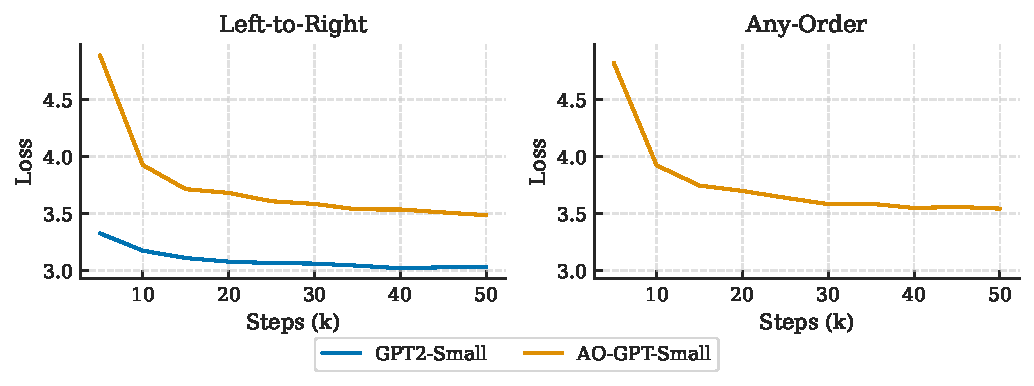
\includegraphics[width=0.8\linewidth]{plots/loss_vs_steps.pdf}
  \caption{Training loss curves comparing a standard AR GPT against an AO-GPT. Both models employ an identical decoder-only architecture, with AO-GPT demonstrating slower initial convergence.}
  \label{fig:loss_vs_steps}
\end{figure}
As established in the preliminaries and further elaborated by NADE~\cite{uria2016neural} and recent analyses such as RADD~\cite{ou2024your}, the training objective for MDMs ($\mathcal{L}_{\text{MDM}}$) is equivalent to that of Any-Order AR models ($\mathcal{L}_{\text{AO-AR}}$). This equivalence can be formally expressed as:
\begin{equation}
\label{eq:mdm_aoar_equivalence}
\begin{aligned}
\mathcal{L}_{\text{MDM}} &= \int_{0}^1 \frac{1}{t} \mathbb{E}_{q_{t|0}\left(\boldsymbol{x}_t | \boldsymbol{x}_0\right)}\left[ \sum_{i:\boldsymbol{x}_0^i = [\text{MASK}]} -\log p_{\boldsymbol{\theta}}(\boldsymbol{x}_0^i|\boldsymbol{x}_t)\right] \mathrm{d}t \\
&\overset{\text{\cite{ou2024your}}}{=} n \cdot \mathbb{E}_{l \sim U(1, \dots, n)} \frac{1}{n - l + 1} \mathbb{E}_{\sigma\sim \mathcal{U}(S_n)} \sum_{r=l}^{n} - \log p_{\theta}(\boldsymbol{x}_{\sigma_r} | \boldsymbol{x}_{\sigma_{<l}})\\
&\overset{\text{\cite{uria2016neural}}}{=} \mathbb{E}_{\sigma\sim \mathcal{U}(S_n)} \left[\sum_{i=1}^n -\log p_{\boldsymbol{\theta}}\left(\boldsymbol{x}_{\sigma_i}|\boldsymbol{x}_{\sigma_{<i}}\right)\right] =\mathcal{L}_{\text{AO-AR}}
\end{aligned}
\end{equation}
This mathematical equivalence is pivotal. It implies that when MDMs (via their AO-AR formulation) and standard AR models are implemented using the same decoder-only architecture, the fundamental difference in their training objectives lies in the distribution over token orders. Standard AR models adhere to a fixed, left-to-right order (i.e., the permutation $\sigma$ is the identity, $\sigma = \text{id}$), while AO-AR models (and thus MDMs) effectively learn by averaging over all possible $n!$ permutations ($\sigma \sim \mathcal{U}(S_n)$). Therefore, the central goal of this section is to investigate the following key question:
\begin{tcolorbox}[
    enhanced,
    colback=LightGoldenrodYellow!40,
    colframe=black!20,
    arc=2mm, 
    boxrule=0.5pt, 
    boxsep=0mm,
    before skip=2mm,
    after skip=2mm
]
\textbf{Question 1:} \textit{Within decoder-only architecture, what are the differences in modeling capabilities and empirical performance when using AR versus MDM formulation for language tasks?}
\end{tcolorbox}
To address Question 1, we first examine the training dynamics of these two approaches when implemented within an identical decoder-only architecture, specifically focusing on their convergence behavior. We train a standard left-to-right AR model and an AO-AR model on the same OpenWebText~\cite{Gokaslan2019OpenWeb} dataset, with exactly the same architecture and model size (standard GPT-2 Small size), and observe their loss progression. Specifically, we simultaneously compare the AR loss~\cref{eq:ar loss} and AO-AR loss~\cref{eq:ao-ar loss}. In the figure, these are labeled `Left-to-Right' and `Any-Order', respectively. Our initial experiments, illustrated in Figure~\ref{fig:loss_vs_steps}, reveal a notable difference in training progression:
\begin{tcolorbox}[
    enhanced,
    colback=LightGoldenrodYellow!40,
    colframe=black!20,
    arc=2mm, 
    boxrule=0.5pt, 
    boxsep=0mm,
    before skip=2mm,
    after skip=2mm
]
\textbf{Finding 1:} \textit{Any-Order GPT converges significantly slower in the initial training stages compared to its standard GPT counterpart when both utilize the same architecture.}
\end{tcolorbox}
This initial observation (Finding 1) suggests that the any-order objective ($\sigma \sim \mathcal{U}(S_n)$), despite its flexibility, might slow initial learning due to increased task complexity compared to the fixed left-to-right ($\sigma = \text{id}$) order. The slower AO-AR convergence could arise from two main factors: (1). \textit{Weight Sharing Burden}: learning representations effective across $n!$ permutations is demanding.
(2). \textit{Prevalence of Less Informative Orders}: many permutations in $\mathcal{U}(S_n)$ might be uninformative.

To further probe the effect of prediction order, we next evaluate model training under conditions where a single, predetermined order is maintained throughout. We compare models trained on: a) conventional left-to-right ($\sigma=\text{id}$), b) a singular, randomly sampled permutation ($\sigma_{\text{rand}} \in S_n$) that remains fixed for the entirety of the training phase, and c) a block-wise permutation strategy, serving as an intermediate approach motivated by Block Diffusion~\cite{arriola2025block}. Globally, this method processes blocks of tokens sequentially from left to right. However, within each block, tokens are processed according to a fixed, non-left-to-right permutation. For example, if the sequence is divided into 4-token blocks, the first block of tokens (indices 0,1,2,3) would be processed in the order $0 \to 2 \to 3 \to 1$. The next block (indices 4,5,6,7) would then be processed as $4 \to 6 \to 7 \to 5$. This specific intra-block permutation remains constant throughout training. Figure~\ref{fig:sec3_combined}(a) presents these results. The comparison in Figure~\ref{fig:sec3_combined}(a) leads to our second finding:
\begin{tcolorbox}[
    enhanced,
    colback=LightGoldenrodYellow!40,
    colframe=black!20,
    arc=2mm, 
    boxrule=0.5pt, 
    boxsep=0mm,
    before skip=2mm,
    after skip=2mm
]
\textbf{Finding 2.1:} \textit{Even when both are trained on only one fixed order, the standard Left-to-Right order converges much faster than an arbitrary, randomly selected fixed order from $S_n$.}

\textbf{Finding 2.2:} \textit{Fixed block-wise random serves as an interpolation between Left-to-Right and purely random order in terms of convergence speed.}
\end{tcolorbox}
\begin{remark}[Identical Loss Lower Bound]
The minimum achievable cross-entropy loss for any autoregressive factorization is the true entropy of the data, $H(\boldsymbol{x})$.
By the chain rule, $H(\boldsymbol{x}) = \sum_{i=1}^n H(\boldsymbol{x}_{\sigma_i} | \boldsymbol{x}_{\sigma_{<i}})$ for any permutation $\sigma \in S_n$.
Thus, the optimal loss value is identical regardless of the chosen generation order (e.g., left-to-right, any fixed random order, or averaged over all orders as in AO-AR).
Differences in convergence or final empirical loss values therefore reflect practical learning challenges and inductive biases under different ordering schemes, not a difference in the achievable target for a perfect model.
This ensures the fairness of our loss comparisons.
\end{remark}
This underscores language's intrinsic left-to-right structure. While order-agnosticism (and thus MDMs) offers flexibility, averaging over all permutations may be less optimal. 
Given the observed slower convergence of purely Any-Order models (Finding 1) and the apparent advantage of the L2R order (Finding 2), a natural question arises: can we retain the flexibility of AO-GPT while mitigating its convergence drawbacks, perhaps by guiding it with some explicit L2R signal?

To explore this, we investigate the effect of incorporating a small fraction of standard Left-to-Right (L2R) ordered data directly into the training process of an AO-GPT. Specifically, we modify the sampling of generation orders $\sigma$ such that 90\% of training instances use an order sampled uniformly from $S_n$ (i.e., $\sigma \sim \mathcal{U}(S_n)$), while the remaining 10\% of instances use the fixed L2R order ($\sigma = \text{id}$). The impact of this hybrid approach on training dynamics and performance is illustrated in Figure~\ref{fig:sec3_combined}(b). Also, as shown in Table~\ref{tab:model ppl} under the "Left-to-Right" evaluation, our AO-GPT model incorporating this 10\% L2R data achieves significantly lower zero-shot validation perplexity compared to a purely any-order one, underscoring the substantial improvement in final loss achieved by this hybrid approach. This experiment yields two significant observations:
\begin{tcolorbox}[
    enhanced,
    colback=LightGoldenrodYellow!40,
    colframe=black!20,
    arc=2mm, 
    boxrule=0.5pt, 
    boxsep=0mm,
    before skip=2mm,
    after skip=2mm
]
\textbf{Finding 3.1:} \textit{Incorporating a small fraction (10\%) of explicitly Left-to-Right ordered data into the training of an AO-GPT drastically improves its performance (both convergence speed and final loss) when evaluated on standard Left-to-Right.}
\end{tcolorbox}
This result, while perhaps not entirely unexpected given the inherent structure of language, is starkly illustrated when comparing final performance metrics. More surprisingly, this hybrid training strategy also benefits the model's any-order capabilities:
\begin{tcolorbox}[
    enhanced,
    colback=LightGoldenrodYellow!40,
    colframe=black!20,
    arc=2mm, 
    boxrule=0.5pt, 
    boxsep=0mm,
    before skip=2mm,
    after skip=2mm
]
\textbf{Finding 3.2:} \textit{A small fraction (10\%) of Left-to-Right data can even improve the model performance on Any-Order data.}
\end{tcolorbox}
Finding 3.2 is particularly intriguing. It suggests that highly structured L2R patterns provide a beneficial inductive bias or a more stable learning signal, helping the model learn fundamental linguistic structures more effectively. This, in turn, appears to enhance generalization across arbitrary permutations, rather than being a mere data trade-off. This phenomenon itself warrants dedicated investigation beyond our initial exploration, as a comprehensive understanding of this benefit is a promising direction for future work.

\begin{figure}[t] % Figure 本身的浮动位置是 [t] (top of page)
    \centering
    \begin{subfigure}[t]{0.34\linewidth} % 改为 [t]
        \centering
        % 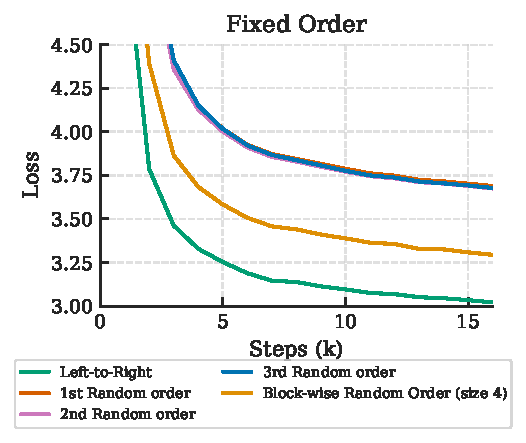
\includegraphics[width=\linewidth]{plots/order.pdf} % 替换为占位符
        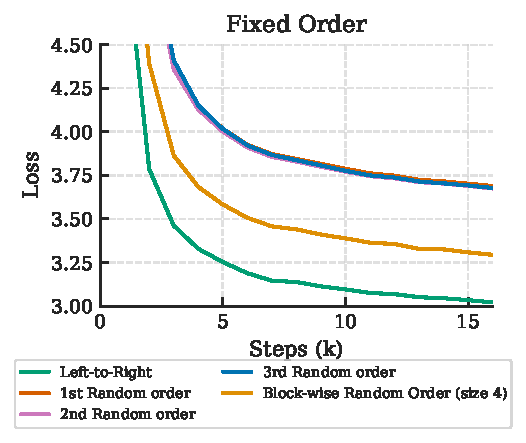
\includegraphics[width=\linewidth, height=4cm, keepaspectratio]{plots/order.pdf} % 使用占位符并设定高度示例
    \end{subfigure}% 注意这里最好不要有换行，或者加一个 % 来避免多余空格
    \begin{subfigure}[t]{0.66\linewidth} % 改为 [t]
        \centering
        % 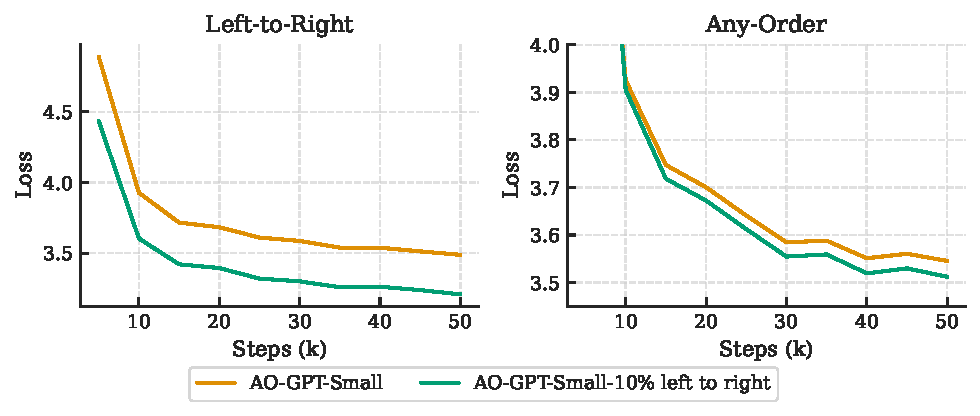
\includegraphics[width=\linewidth]{plots/plus_ar_loss.pdf}
        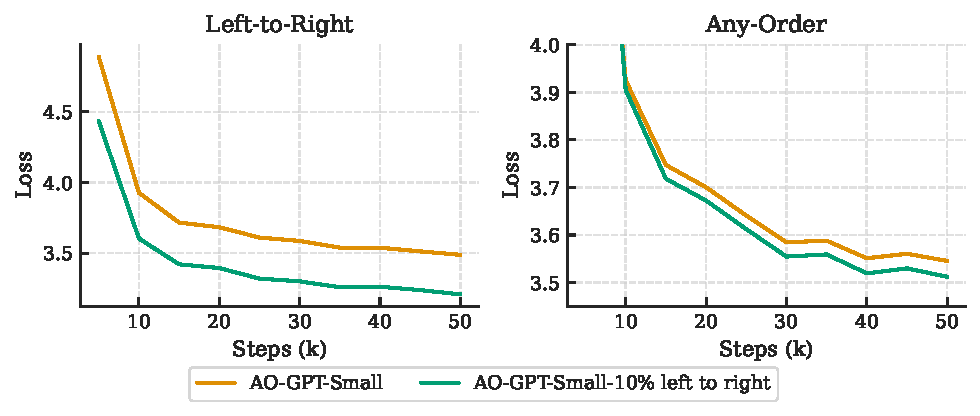
\includegraphics[width=\linewidth, height=4.3cm, keepaspectratio]{plots/plus_ar_loss.pdf} % 使用占位符并设定高度示例
    \end{subfigure}
    % \vspace{-3mm}
    \caption{(a) Convergence speed with different fixed prediction orders: left-to-right, fixed random, and fixed block-wise random. (b) Impact of adding 10\% left-to-right (L2R) data to AO-GPT training on its L2R and any-order loss.}
    \label{fig:sec3_combined}
\end{figure}
\section{Comparing Encoder-Only and Decoder-Only for Masked Diffusion Models}
\label{sec:mdm encoder decoder}
Building on the insights from comparing AR and AO-AR within a decoder-only framework, we now turn our attention to the impact of the architectural choice itself when implementing an Any-Order Autoregressive (or Masked Diffusion Model) formulation. This leads to our second question:
\begin{tcolorbox}[
    enhanced,
    colback=LightGoldenrodYellow!40,
    colframe=black!20,
    arc=2mm, 
    boxrule=0.5pt, 
    boxsep=0mm,
    before skip=2mm,
    after skip=2mm
]
\textbf{Question 2:} \textit{Within the MDM framework for language tasks, what are the theoretical and empirical differences when selecting an encoder-only versus a decoder-only architecture?}
\end{tcolorbox}
To address Question 2, we analyze how encoder-only and decoder-only architectures differ in modeling the univariate conditional probabilities $p(\boldsymbol{x}_j | \boldsymbol{x}_{E})$ that underpin AO-AR or MDM, where $j$ is the index of the target token and $E \subset \{1, \ldots, n\} \setminus \{j\}$ is the index set of observed context tokens $\boldsymbol{x}_{E}$.
\subsection{Modeling Univariate Conditional Probabilities}
\label{sec:modeling_conditionals} % 
\textbf{Order-Invariant Formulation:} For encoder-only AO-AR, the computed conditional probability $p_{\boldsymbol{\theta}}(\boldsymbol{x}_j | \boldsymbol{x}_{E})$ is \textit{order-invariant}. Provided that each token in $\boldsymbol{x}_{E}$ is correctly paired with its positional encoding, the permutation of these token-position pairs within the input does not alter the output probability for $\boldsymbol{x}_j$.

\textbf{Order-Dependent Formulation:} For decoder-only AO-AR, the inherent asymmetry in causal attention means the prediction $p_{\boldsymbol{\theta}}(\boldsymbol{x}_j | \boldsymbol{x}_{E}, \sigma_{E})$ is \textit{order-dependent} even each token in $\boldsymbol{x}_{E}$ is correctly paired with its positional encoding. The probability explicitly depends on the sequence $\sigma_{E}$ in which the context tokens $\boldsymbol{x}_{E}$ are presented to the model.

Henceforth, we refer to $p_{\boldsymbol{\theta}}(\boldsymbol{x}_j | \boldsymbol{x}_{E})$ as an \textit{order-invariant} conditional probability and $p_{\boldsymbol{\theta}}(\boldsymbol{x}_j | \boldsymbol{x}_{E}, \sigma_{E})$ as an \textit{order-dependent} conditional probability. The distinction between order-invariant and order-dependent modeling leads to different counts of the effective conditional probability space covered by each architecture.
\begin{tcolorbox}[
    enhanced,
    colback=LightGoldenrodYellow!40,
    colframe=black!20,
    arc=2mm, 
    boxrule=0.5pt, 
    boxsep=0mm,
    before skip=2mm,
    after skip=2mm
]
\textbf{Finding 4:} \textit{Encoder-only AO-AR models $n\cdot2^{n-1}$ order-invariant univariate conditional probability while decoder-only AO-AR models approximately $e\cdot n!$ order-dependent univariate conditional probability.}
\end{tcolorbox}
\textbf{Encoder-only AO-AR:} This architecture models the probability of predicting any token $\boldsymbol{x}_j$ ($n$ possibilities) given any subset $\boldsymbol{x}_E$ of the other $n-1$ tokens. Since the order of $\boldsymbol{x}_E$ does not matter, we count the number of distinct pairs $(j, E)$. For each target $j$, there are $2^{n-1}$ possible subsets $E$. Therefore, the model represents $n \cdot 2^{n-1}$ unique \textit{order-invariant} conditional probabilities. This quantity can be derived combinatorially: summing over all possible context sizes $k$ (from $0$ to $n-1$), we choose $k$ context tokens ($\binom{n}{k}$ ways) and have $n-k$ possible target tokens. The total is $\sum_{k=0}^{n-1} \binom{n}{k} (n-k) = n \cdot 2^{n-1}$.

\textbf{Decoder-only AO-AR:} This architecture models \textit{order-dependent} probabilities. While it can potentially generate samples according to any of the $n!$ permutations, the fundamental units are $p_{\boldsymbol{\theta}}(\boldsymbol{x}_j | \boldsymbol{x}_{E}, \sigma_{E})$. To count the number of distinct such terms, we again sum over context size $k$. For a fixed context set $E$ of size $k$ and a fixed target $j$, there are $k!$ possible orderings $\sigma_E$. Therefore, the total number of distinct order-dependent probabilities is:
\begin{align}
N_{\text{ordered}} &= \sum_{k=0}^{n-1} \underbrace{\binom{n}{k}}_{\substack{\text{Choose} \\ \text{context}}} \underbrace{(n-k)}_{\substack{\text{Choose} \\ \text{target}}} \underbrace{k!}_{\substack{\text{Order} \\ \text{context}}} = \sum_{k=0}^{n-1} \frac{n!}{k!(n-k)!} (n-k) k! = n! \sum_{i=0}^{n-1} \frac{1}{i!}\label{eq:decoder_count_sum}
\end{align}
As $n \to \infty$, this sum quickly converges to $e \cdot n!$. This significantly larger number compared to the encoder-only case reflects the decoder's sensitivity to the permutation of the context. The core difference highlighted by these counts is whether the model's prediction $p(\boldsymbol{x}_j | \dots)$ is conditioned on the context as an unordered set $\boldsymbol{x}_E$ (encoder) or as an ordered sequence $(\boldsymbol{x}_{\sigma_E(1)}, \dots, \boldsymbol{x}_{\sigma_E(k)})$ (decoder).
\subsection{Ensemble on Context Order}
\begin{table}\small
  \caption{Zero-shot validation perplexity($\downarrow$) on a variety of datasets on GPT-2-medium sized models ($\sim$350M). $^\dagger$Model reproduced by the authors. $^\ddagger$Model trained with an additional 10\% left-to-right ordered data.}
  \label{tab:model ppl}
  \centering
  \begin{tabular}{@{}l ccccc@{}}
    \toprule
    \textbf{Model} & \textbf{LAMBADA} & \textbf{WikiText2} & \textbf{PTB} & \textbf{WikiText103} & \textbf{1BW} \\
    \midrule

    % --- Encoder-only Models ---
    \multicolumn{6}{@{}l}{\textit{Left-to-Right}} \\ % Header spans all 6 columns
    % \addlinespace % Optional extra space
    \multicolumn{6}{@{}l}{\textit{\quad Encoder-only Models}} \\ % Indented sub-header
    % \addlinespace % Optional extra space
    \quad\quad SEDD & 39.19 & 30.29& 88.18&30.05& 53.54 \\
    \quad\quad RADD & \textbf{38.60} & \textbf{29.71} &\textbf{76.00} &\textbf{29.96} & \textbf{52.36} \\
    % \addlinespace
    \multicolumn{6}{@{}l}{\textit{\quad Decoder-only Models}} \\ % Indented sub-header
    % \addlinespace % Optional extra space
    \quad\quad GPT-2  & \textbf{35.66} & 31.80 & 123.14&31.39&55.72\\
    \quad\quad $\sigma$-GPT$^\dagger$ &61.05 &44.80 &121.48&43.68&76.74\\
    \quad\quad \textit{AO-GPT$^\ddagger$}&42.44 &\textbf{31.52}&\textbf{87.56}&\textbf{30.86}& \textbf{50.23} \\
    \midrule % Separator between major categories
    \multicolumn{6}{@{}l}{\textit{Any-Order}} \\
    % \addlinespace
    \multicolumn{6}{@{}l}{\textit{\quad Encoder-only Models}} \\
    % \addlinespace % Optional extra space
    \quad\quad SEDD &42.77&31.04&87.12&29.98&61.19\\
    \quad\quad RADD&\textbf{41.96}&\textbf{29.96}&\textbf{79.06}&\textbf{28.51}&\textbf{57.07}\\
    % \addlinespace
    \multicolumn{6}{@{}l}{\textit{\quad Decoder-only Models}} \\
    % \addlinespace % Optional extra space
    \quad\quad $\sigma$-GPT$^\dagger$  &57.27 &43.28&126.11 &41.80 & 74.81 \\
    \quad\quad \textit{AO-GPT$^\ddagger$}  &49.79&33.73&101.01 &32.38&65.90\\
    \quad\quad \textit{AO-GPT$^\ddagger$ + Ensembles} ($8$ times) &45.08&30.63 &87.74&29.46&59.11 \\
    \quad\quad \textit{AO-GPT$^\ddagger$ + Ensembles} ($64$ times) &\textbf{44.31}&\textbf{30.16} &\textbf{85.75}&\textbf{28.98}&\textbf{58.18}\\
    \bottomrule
  \end{tabular}
\end{table}
As shown in Figure~\ref{fig:ppl ensemble} (Ensemble Times $=1$), decoder-only AO-AR models exhibit higher zero-shot perplexity than their encoder-only counterparts. We hypothesize this performance gap is due to the inherently harder task faced by decoders: they must learn to represent approximately $e \cdot n!$ distinct order-dependent conditional probabilities, a vastly larger space than the $n \cdot 2^{n-1}$ order-invariant conditionals modeled by encoders. To verify this, given that the increased number is completely due to the order of context tokens $\boldsymbol{x}_{\sigma_{<i}}$, we introduce an ensembling technique for evaluating $\mathcal{L}_{\text{AO-AR}} = \mathbb{E}_{\sigma\sim \mathcal{U}(S_n)} \left[\sum_{i=1}^n -\log p_{\boldsymbol{\theta}}\left(\boldsymbol{x}_{\sigma_i}|\boldsymbol{x}_{\sigma_{<i}}\right)\right]$. For each individual conditional probability $p_{\boldsymbol{\theta}}\left(\boldsymbol{x}_{\sigma_i}|\boldsymbol{x}_{\sigma_{<i}}\right)$, we generate $M$ random permutations of the context sequence $\boldsymbol{x}_{\sigma_{<i}}$. The probability used for the loss calculation, $p_{\text{ens}}(\boldsymbol{x}_{\sigma_i}|\boldsymbol{x}_{\sigma_{<i}})$, is obtained by averaging the model's predictions across $M$ permutations of the context $\boldsymbol{x}_{\sigma_{<i}}$:
\begin{equation}
p_{\text{ens}}(\boldsymbol{x}_{\sigma_i}|\boldsymbol{x}_{\sigma_{<i}}) = \frac{1}{M} \sum_{j=1}^{M} p_{\boldsymbol{\theta}}\left(\boldsymbol{x}_{\sigma_i}|\boldsymbol{x}_{\text{perm}_j(\sigma_{<i})}, \text{perm}_j(\sigma_{<i})\right).
\end{equation}
Here, $\text{perm}_j$ signifies the $j$-th permutation of the context sequence. (We always include the identity permutation among the $M$ permutations in practice.) Crucially, while the order of the input sequence fed to the model is permuted, each token remains associated with its original positional encoding. This averaging process approximates the order-invariance of an encoder by marginalizing over the context order. The results in Figure~\ref{fig:ppl ensemble} show that the ensemble on order context fills the gap.
\begin{figure}[t]
  \centering
  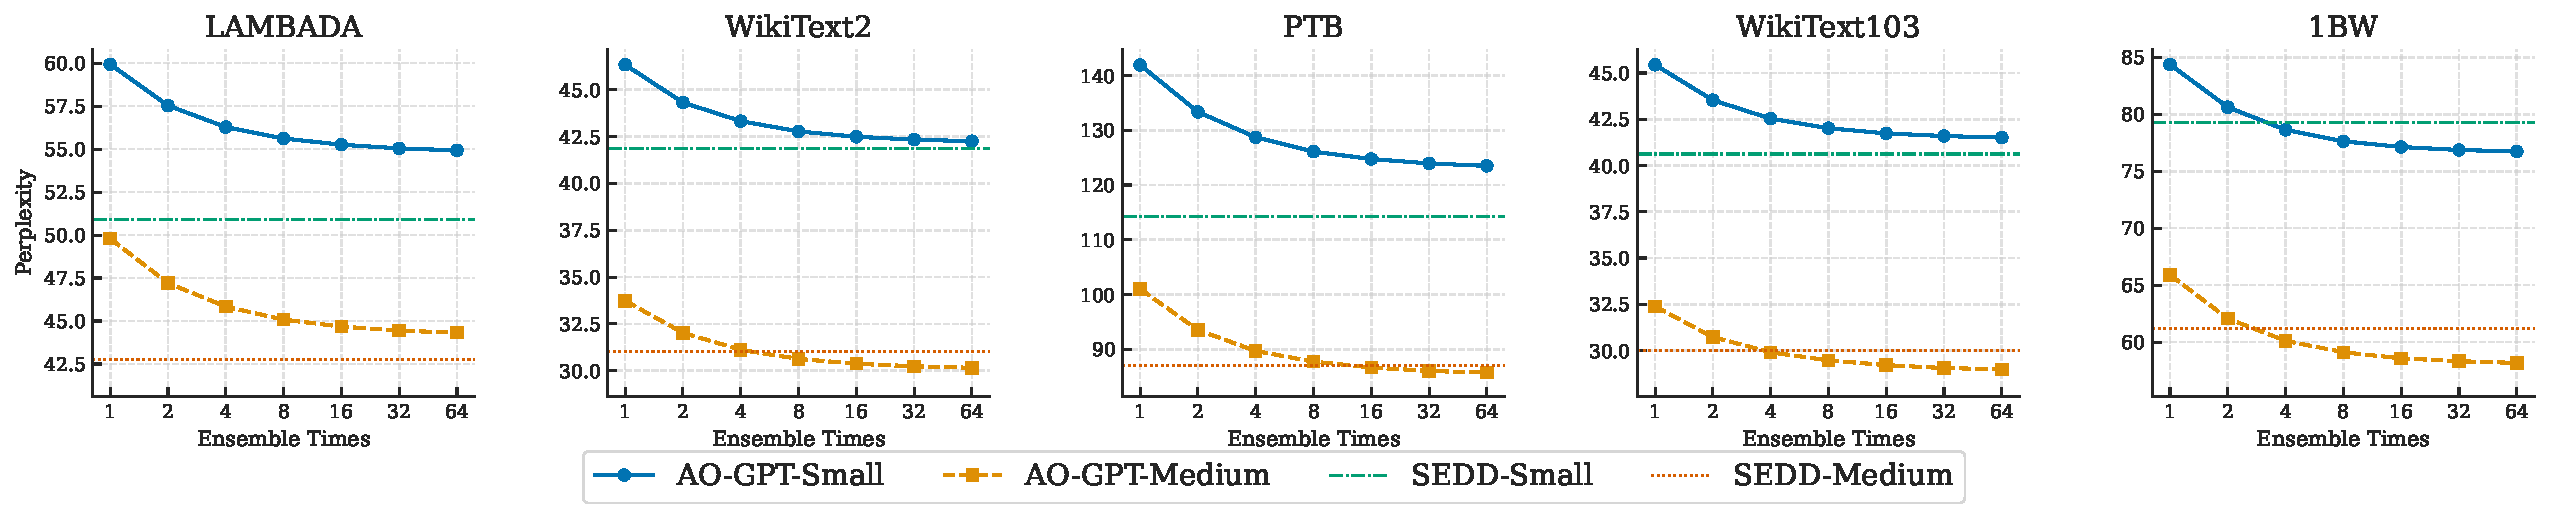
\includegraphics[width=1.0\linewidth]{plots/perplexity_vs_ensemble_1x5.pdf}
  \caption{Zero-shot unconditional perplexity (↓) for varying ensemble sizes. An ensemble size of 1 represents the baseline model without ensembling.}
  \label{fig:ppl ensemble}
\end{figure}


\begin{tcolorbox}[
    enhanced,
    colback=LightGoldenrodYellow!40,
    colframe=black!20,
    arc=2mm, 
    boxrule=0.5pt, 
    boxsep=0mm,
    before skip=2mm,
    after skip=2mm
]
\textbf{Finding 5:} \textit{Decoder-only AO-AR falls short of their Encoder-only counterpart, while ensemble on order context fills the gap.}
\end{tcolorbox}

This observation validates our initial hypothesis. The dramatic reduction in perplexity, which brings the decoder's performance nearly in line with the encoder-only models, confirms that this sensitivity to context order is the dominant reason for the initial performance gap.

\subsection{Generation Computational Complexity}
The reverse process in MDMs iteratively recovers masked tokens as follows:
\begin{equation}\label{eq:q_st_definition_main}
q_{s|t} = \prod_{i=0}^{n-1} q_{s|t}(\boldsymbol{x}_s^i|\boldsymbol{x}_t),\text{where } q_{s|t}(\boldsymbol{x}_s^i|\boldsymbol{x}_t)=\begin{cases}
1, & \boldsymbol{x}_t^i \neq [\text{MASK}], \boldsymbol{x}_s^i = \boldsymbol{x}_t^i \\
\frac{s}{t}, & \boldsymbol{x}_t^i = [\text{MASK}], \boldsymbol{x}_s^i = [\text{MASK}] \\
\frac{t-s}{t} q_{0|t}(\boldsymbol{x}_s^i | \boldsymbol{x}_t), & \boldsymbol{x}_t^i = [\text{MASK}], \boldsymbol{x}_s^i \neq [\text{MASK}].
\end{cases}
\end{equation}
\begin{figure}[h] 
  \centering
  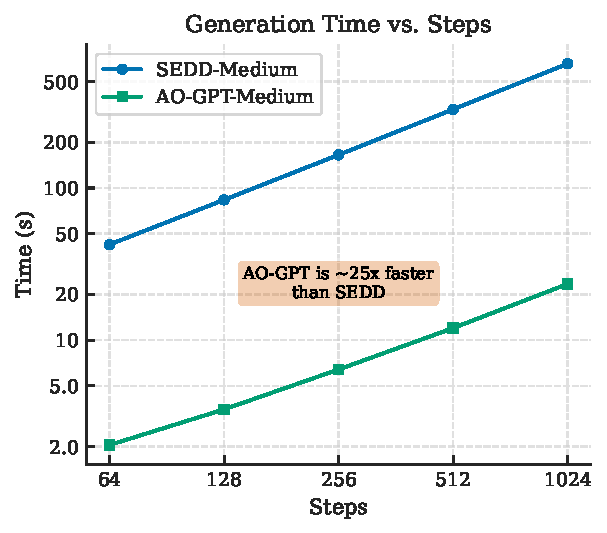
\includegraphics[width=0.5\linewidth]{plots/steps_vs_time_plot_enhanced.pdf} % Image width relative to wrapfigure width
  \caption{Generation time versus number of generation steps with sequence length $1024$ and batch size$=32$ for decoder-only AO-AR models (with KV-cache and Lemma~\ref{lemma:efficient_sampling}) and their encoder-only counterparts (SEDD).}
  \label{fig:generation_speed_comparison}
\end{figure}
Here, $q_{0|t}(\boldsymbol{x}_s^i | \boldsymbol{x}_t)$ (when $\boldsymbol{x}_t^i = [\text{MASK}]$) represents a distribution over the vocabulary for predicting a non-$[\text{MASK}]$ token. Sampling $\boldsymbol{x}_s$ from $q_{s|t}(\boldsymbol{x}_s|\boldsymbol{x}_t)$ involves sampling each $\boldsymbol{x}_s^i$ independently. For positions $i$ where $\boldsymbol{x}_t^i \neq [\text{MASK}]$, $\boldsymbol{x}_s^i$ is deterministically set to $\boldsymbol{x}_t^i$. For positions where $\boldsymbol{x}_t^i = [\text{MASK}]$, a more efficient two-stage sampling procedure can be employed, as stated in Lemma \ref{lemma:efficient_sampling}.
\begin{lemma}[Efficient Sampling Algorithm] \label{lemma:efficient_sampling}
For sampling $\boldsymbol{x}_s^i$ from $q_{s|t}(\boldsymbol{x}_s^i|\boldsymbol{x}_t)$ as defined in Equation \eqref{eq:q_st_definition_main} when $\boldsymbol{x}_t^i = [\text{MASK}]$, an equivalent sampling procedure is:

\hspace{10mm} 1. Sample a binary variable $b \sim \text{Bernoulli}\left(\frac{s}{t}\right)$.

\hspace{10mm} 2. If $b=1$, set $\boldsymbol{x}_s^i = [\text{MASK}]$.

\hspace{10mm} 3. If $b=0$, sample $\boldsymbol{x}_s^i$ from the distribution $q_{0|t}(\cdot | \boldsymbol{x}_t)$.
% This procedure is mathematically equivalent to directly sampling from $q_{s|t}(\boldsymbol{x}_s^i|\boldsymbol{x}_t)$. 
It reduces computational cost by only requiring the evaluation of $q_{0|t}(\cdot | \boldsymbol{x}_t)$ when $b=0$. The proof of equivalence and a detailed discussion of the computational benefits are provided in Appendix \ref{appendix:proof_lemma1}.
\end{lemma}
Leveraging both the KV-cache mechanism and the efficient sampling technique from Lemma \ref{lemma:efficient_sampling}, decoder-only AO-AR models significantly reduce per-step computational costs. At each generation step, the KV-cache obviates recomputing context tokens, while efficient sampling (Lemma \ref{lemma:efficient_sampling}) restricts computation to only those tokens designated for unmasking. This synergy reduces the computational complexity of each step to $O(1)$, a marked advantage over their encoder-only counterparts. Our findings are summarized as follows:
\begin{tcolorbox}[
    enhanced,
    colback=LightGoldenrodYellow!40,
    colframe=black!20,
    arc=2mm, 
    boxrule=0.5pt, 
    boxsep=0mm,
    before skip=2mm,
    after skip=2mm
]
\textbf{Finding 6:} \textit{The total computational complexity of generating a length $n$ sequence using an encoder-only AO-AR is $O(n^2)$; with both KV-cache and \Cref{lemma:efficient_sampling}, a decoder-only AO-AR's computational complexity is $O(n)$.}
\end{tcolorbox}
The $O(n)$ total complexity for decoder-only AO-AR models (Finding 7) translates directly into tangible performance gains. This theoretical advantage is empirically validated by the significant generation speedups visualized in Figure \ref{fig:generation_speed_comparison}. Beyond speed, we also evaluated the unconditional generation perplexity. To ensure a fair comparison and address the observation by~\cite{zheng2024masked} that \texttt{float32} Gumbel noise (as used in SEDD~\cite{lou2023discrete}) can lower effective temperature, we utilized \texttt{float64}. We then compared AO-GPT and SEDD under three distinct annealing configurations: 1) no annealing (Top-p 1.0, Temperature 1.0), 2) mild annealing (Top-p 0.95, Temperature 0.9), and 3) appropriate annealing (Top-p 0.95, Temperature 0.7). The detailed results of generation perplexity are in Table~\ref{tab:perplexity_generation}, with the main conclusions summarized in Findings 8.1 and 8.2.
\begin{tcolorbox}[
    enhanced,
    colback=LightGoldenrodYellow!40,
    colframe=black!20,
    arc=2mm, 
    boxrule=0.5pt, 
    boxsep=0mm,
    before skip=2mm,
    after skip=2mm
]
\textbf{Finding 7.1:} \textit{AO-GPT can achieve $~25\times$ speedup on generation compared with SEDD.}

\textbf{Finding 7.2:} \textit{AO-GPT exhibits higher generation perplexity without logit annealing, while appropriate annealing brings its perplexity to a comparable level.}
\end{tcolorbox}

The observed perplexity difference, particularly without annealing (Finding 8.2), can be attributed to AO-GPT's lower modeling likelihood compared to SEDD when considered in non-ensembled configurations. Thus, while SEDD might achieve better perplexity for models of comparable size, AO-GPT's striking ~25x speed advantage (Finding 8.1) presents a compelling trade-off between generation quality and practical inference speed. The findings in this section illuminate the significant distinctions between encoder-centric and decoder-centric approaches, suggesting that exploring how to synergistically combine their respective advantages is a crucial direction for future work.
% \begin{figure}[htbp]
%   \centering
%   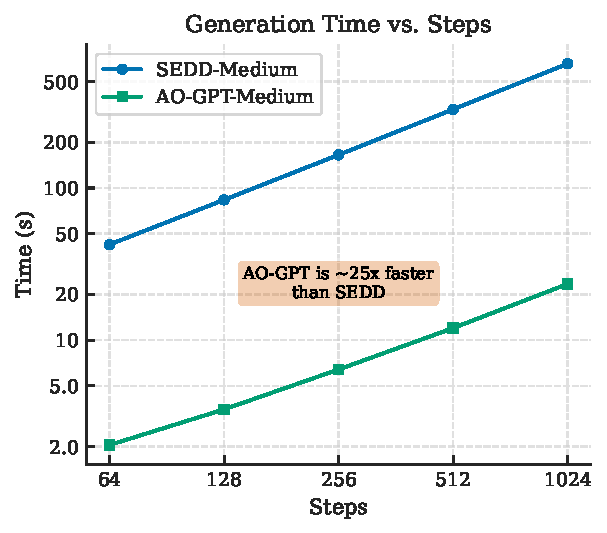
\includegraphics[width=0.5\linewidth]{plots/steps_vs_time_plot_enhanced.pdf}
%   \caption{Generation time versus number of generation steps under sequence length $1024$ for decoder-only AO-AR models (with KV-cache and Lemma~\ref{lemma:efficient_sampling}) and their encoder-only counterparts (SEDD).}
%   \label{fig:generation_speed_comparison}
% \end{figure}

\begin{table}[t]\small
  \caption{Generation Perplexity measured by GPT-2-Large of AO-GPT-Medium and SEDD-Medium across different generation steps and sampling settings (Top-p and Temperature). Lower values are better.}
  \label{tab:perplexity_generation} % Changed label
  \centering
  % Using 'r' (right-aligned) for numerical columns.
  % Headers for these columns are centered using \multicolumn{1}{c}{...}
  \begin{tabular}{@{}ll r r r r r@{}}
    \toprule
    \multicolumn{2}{@{}c}{\textbf{Sampling Setting}} & \multicolumn{5}{c}{\textbf{Steps}} \\
    \cmidrule(lr){1-2} \cmidrule(lr){3-7}
    {\textit{\shortstack[l]{Top-p \\ Temperature}}} & {\textit{Model}} &
    \multicolumn{1}{c}{64} & \multicolumn{1}{c}{128} &
    \multicolumn{1}{c}{256} & \multicolumn{1}{c}{512} &
    \multicolumn{1}{c}{1024} \\
    \midrule
    % Setting 1: top-p=1.0, temp=1.0
    \multirow{2}{*}{1.0, 1.0} & AO-GPT & 194.588 & 154.837 & 148.006 & 140.369 & 136.406 \\
                              & SEDD   & 121.574 & 100.014 &  86.428 &  87.666 &  81.689 \\
    \midrule
    % Setting 2: top-p=0.95, temp=0.9
    \multirow{2}{*}{0.95, 0.9} & AO-GPT & 33.528 & 29.359 & 27.378 & 27.020 & 26.952 \\
                               & SEDD   & 25.414 & 22.034 & 19.481 & 19.022 & 19.311 \\
    \midrule
    % Setting 3: top-p=0.95, temp=0.7
    \multirow{2}{*}{0.95, 0.7} & AO-GPT & 6.105 & 5.615 & 5.507 & 5.095 & 4.611 \\
                               & SEDD   & 6.400 & 6.042 & 5.201 & 4.979 & 5.051 \\
    \bottomrule
  \end{tabular}
  % \vspace{-4mm}
\end{table}



